\documentclass[aspectratio=43]{beamer}
% \documentclass[aspectratio=169]{beamer}

% Title --------------------------------------------
\title{\Huge Introduction}
\author{Francisco Villamil}
\date{War, peace, and political violence\\UC3M, Fall 2023}

%%% NOTE -- CHECK THIS: https://github.com/paulgp/beamer-tips


%%% Building heavily on https://github.com/kylebutts/templates

% xcolor, define them
\usepackage{xcolor}

% TEXT COLORS
\definecolor{red}{HTML}{9a2515}
\definecolor{yellow}{HTML}{EBC944}
\definecolor{asher}{HTML}{555F61}
\definecolor{jet}{HTML}{131516}

% THEME COLORS
\definecolor{accent}{HTML}{107895}
\definecolor{accent2}{HTML}{9a2515}

% Color commands
\newcommand\red[1]{{\color{red}#1}}
\newcommand\yellow[1]{{\color{yellow}#1}}
\newcommand\asher[1]{{\color{asher}#1}}

\newcommand\BGred[1]{{\colorbox{red!80!white}{#1}}}
\newcommand\BGyellow[1]{{\colorbox{yellow!80!white}{#1}}}
\newcommand\BGasher[1]{{\colorbox{asher!80!white}{#1}}}

\renewcommand<>{\BGyellow}[1]{\only#2{\beameroriginal{\BGyellow}}{#1}}

% Appendix numbering
\usepackage{appendixnumberbeamer}

% Beamer Options -------------------------------------

% Background
\setbeamercolor{background canvas}{bg = white}

% Change text margins
\setbeamersize{text margin left = 25pt, text margin right = 15pt}

% \alert
\setbeamercolor{alerted text}{fg = accent2}

% Frame title
\setbeamercolor{frametitle}{bg = white, fg = jet}
\setbeamercolor{framesubtitle}{bg = white, fg = accent}
\setbeamerfont{framesubtitle}{size = \small, shape = \itshape}

% Block
\setbeamercolor{block title}{fg = white, bg = accent2}
\setbeamercolor{block body}{fg = jet, bg = jet!10!white}

% Title page
\setbeamercolor{title}{fg = jet}
\setbeamercolor{subtitle}{fg = accent}

%% Custom \maketitle and \titlepage
\setbeamertemplate{title page}
{
    \begin{centering}
      % \vspace{20mm}
      {\Large \usebeamerfont{title}\usebeamercolor[fg]{title}\inserttitle}\\ \vskip0.25em%
      \ifx\insertsubtitle\@empty%
      \else%
        {\usebeamerfont{subtitle}\usebeamercolor[fg]{subtitle}\insertsubtitle\par}%
      \fi%
      {\vspace{10mm}\insertauthor}\\
      \ifx\insertinstitute\@empty%
      \else%
        {\vspace{5mm}\color{asher}\scriptsize{\insertinstitute}}
      \fi%
      {\color{asher}\small{\insertdate}}\\
    \end{centering}
}

% Table of Contents
\setbeamercolor{section in toc}{fg = accent!70!jet}
\setbeamercolor{subsection in toc}{fg = jet}

% Button
\setbeamercolor{button}{bg = accent}

% Remove navigation symbols
\setbeamertemplate{navigation symbols}{}

% Table and Figure captions
\setbeamercolor{caption}{fg=jet!70!white}
\setbeamercolor{caption name}{fg=jet}
\setbeamerfont{caption name}{shape = \itshape}

% Put slide number / total slides at the bottom right
\makeatother
\makeatletter
\setbeamertemplate{footline} %{\hfill\insertframenumber/\inserttotalframenumber}
{%
  \leavevmode%
  \hbox{
  \begin{beamercolorbox}[wd=\paperwidth,ht=2.5ex,dp=1.125ex,leftskip=.3cm,rightskip=.3cm plus1fil]{footlinecolor}%
    \color{asher}{\hfill\insertframenumber/\inserttotalframenumber}
  \end{beamercolorbox}}%
  \vskip0pt%
}
\makeatother
\makeatletter

% Bullet points

%% Fix left-margins
\settowidth{\leftmargini}{\usebeamertemplate{itemize item}}
\addtolength{\leftmargini}{\labelsep}

%% enumerate item color
\setbeamercolor{enumerate item}{fg = accent}
\setbeamerfont{enumerate item}{size = \small}
\setbeamertemplate{enumerate item}{\insertenumlabel.}

%% itemize
\setbeamercolor{itemize item}{fg = accent!70!white}
\setbeamerfont{itemize item}{size = \small}
\setbeamertemplate{itemize item}[circle]
\setlength{\itemsep}{0pt plus 6pt}

%% right arrow for subitems
\setbeamercolor{itemize subitem}{fg = accent!60!white}
\setbeamerfont{itemize subitem}{size = \small}
\setbeamertemplate{itemize subitem}{$\rightarrow$}

\setbeamertemplate{itemize subsubitem}[square]
\setbeamercolor{itemize subsubitem}{fg = jet}
\setbeamerfont{itemize subsubitem}{size = \small}

% References

%% Bibliography Font, roughly matching aea
\setbeamerfont{bibliography item}{size = \footnotesize}
\setbeamerfont{bibliography entry author}{size = \footnotesize, series = \bfseries}
\setbeamerfont{bibliography entry title}{size = \footnotesize}
\setbeamerfont{bibliography entry location}{size = \footnotesize, shape = \itshape}
\setbeamerfont{bibliography entry note}{size = \footnotesize}

\setbeamercolor{bibliography item}{fg = jet}
\setbeamercolor{bibliography entry author}{fg = accent!60!jet}
\setbeamercolor{bibliography entry title}{fg = jet}
\setbeamercolor{bibliography entry location}{fg = jet}
\setbeamercolor{bibliography entry note}{fg = jet}

%% Remove bibliography symbol in slides
\setbeamertemplate{bibliography item}{}





% Links ----------------------------------------------

\usepackage{hyperref}
\hypersetup{
  colorlinks = true,
  linkcolor = accent,
  filecolor = accent,
  urlcolor = accent,
  citecolor = accent,
}


% Line spacing --------------------------------------
\usepackage{setspace}
\setstretch{1.2}


% \begin{columns} -----------------------------------
\usepackage{multicol}


% % Fonts ---------------------------------------------
% % Beamer Option to use custom fonts
% \usefonttheme{professionalfonts}
%
% % \usepackage[utopia, smallerops, varg]{newtxmath}
% % \usepackage{utopia}
% \usepackage[sfdefault,light]{roboto}
%
% % Small adjustments to text kerning
% \usepackage{microtype}



% Remove annoying over-full box warnings -----------
\vfuzz2pt
\hfuzz2pt


% Table of Contents with Sections
\setbeamerfont{myTOC}{series=\bfseries, size=\Large}
\AtBeginSection[]{
        \frame{
            \frametitle{Roadmap}
            \tableofcontents[current]
        }
    }


% References ----------------------------------------
\usepackage[
    citestyle= authoryear,
    style = authoryear,
    natbib = true,
    backend = biber
]{biblatex}

% Smaller font-size for references
\renewcommand*{\bibfont}{\small}

% Remove "In:"
\renewbibmacro{in:}{}

% Color citations for slides
\newenvironment{citecolor}
    {\footnotesize\begin{color}{accent2}}
    {\end{color}}

\newcommand{\citetcolor}[1]{{\footnotesize\textcolor{asher}{\citet{#1}}}}
\newcommand{\citepcolor}[1]{{\footnotesize\textcolor{asher}{\citep{#1}}}}

% Tables -------------------------------------------
% Tables too big
% \begin{adjustbox}{width = 1.2\textwidth, center}
\usepackage{adjustbox}
\usepackage{array}
\usepackage{threeparttable, booktabs, adjustbox}

% Fix \input with tables
% \input fails when \\ is at end of external .tex file

\makeatletter
\let\input\@@input
\makeatother

% Tables too narrow
% \begin{tabularx}{\linewidth}{cols}
% col-types: X - center, L - left, R -right
% Relative scale: >{\hsize=.8\hsize}X/L/R
\usepackage{tabularx}
\newcolumntype{L}{>{\raggedright\arraybackslash}X}
\newcolumntype{R}{>{\raggedleft\arraybackslash}X}
\newcolumntype{C}{>{\centering\arraybackslash}X}

% Figures

% \imageframe{img_name} -----------------------------
% from https://github.com/mattjetwell/cousteau
\newcommand{\imageframe}[1]{%
    \begin{frame}[plain]
        \begin{tikzpicture}[remember picture, overlay]
            \node[at = (current page.center), xshift = 0cm] (cover) {%
                \includegraphics[keepaspectratio, width=\paperwidth, height=\paperheight]{#1}
            };
        \end{tikzpicture}
    \end{frame}%
}

% subfigures
\usepackage{subfigure}


% Highlight slide -----------------------------------
% \begin{transitionframe} Text \end{transitionframe}
% from paulgp's beamer tips
\newenvironment{transitionframe}{
    \setbeamercolor{background canvas}{bg=accent!60!black}
    \begin{frame}\color{accent!10!white}\LARGE\centering
}{
    \end{frame}
}


% Table Highlighting --------------------------------
% Create top-left and bottom-right markets in tabular cells with a unique matching id and these commands will outline those cells
\usepackage[beamer,customcolors]{hf-tikz}
\usetikzlibrary{calc}
\usetikzlibrary{fit,shapes.misc}

% To set the hypothesis highlighting boxes red.
\newcommand\marktopleft[1]{%
    \tikz[overlay,remember picture]
        \node (marker-#1-a) at (0,1.5ex) {};%
}
\newcommand\markbottomright[1]{%
    \tikz[overlay,remember picture]
        \node (marker-#1-b) at (0,0) {};%
    \tikz[accent!80!jet, ultra thick, overlay, remember picture, inner sep=4pt]
        \node[draw, rectangle, fit=(marker-#1-a.center) (marker-#1-b.center)] {};%
}


\begin{document}

\begin{frame}
  \titlepage
\end{frame}

\begin{frame}
\frametitle{Main focus}
\centering

\begin{itemize}[<+->]
\item Political violence: what is this?
\item Types
\item `Grand events` vs isolated events
\item Connecting logics
\item What, why, how?
\end{itemize}

\end{frame}


% ----------------------------------------------------
\imageframe{img/russia_genocide}
% ----------------------------------------------------

% ----------------------------------------------------
\imageframe{img/russia_terrorist}
% ----------------------------------------------------

\begin{frame}
\frametitle{Course outline}
\centering

\begin{tabular}{lll}
  \asher{\textbf{Week 1}} & \asher{(Sept 7-8)} & \asher{Introduction} \\
  \textbf{Week 2} & (Sept 14-15) & \BGyellow<2>{Basics of IR} \\
  \textbf{Week 3} & (Sept 21-22) & \BGyellow<3>{Interstate wars} \\
  \textbf{Week 4} & (Sept 28-29) & \BGyellow<4>{War throughout history} \\
  \textbf{Week 5} & (Oct 5-6)    & \BGyellow<5>{Civil wars I} \\
  \textbf{Week 6} & (Oct 19-20)  & \BGyellow<5>{Civil wars II} \\
  \textbf{Week 7} & (Oct 26-27)  & \BGyellow<6>{Wartime violence} \\
  \textbf{Week 8} & (Nov 2-3)    & \BGyellow<7>{Rebels and civilians} \\
  \textbf{Week 9} & (Nov 9-10)   & \BGyellow<8>{Terrorism} \\
  \textbf{Week 10} & (Nov 16-17)  & \BGyellow<9>{Postwar and prevention} \\
  \textbf{Week 11} & (Nov 23-24)  & \BGyellow<10>{Transitional Justice} \\
  \textbf{Week 12} & (Nov 30-31)  & \BGyellow<11>{Conflict legacies} \\
  \asher{\textbf{Week 13}} & \asher{(Dec 14-15)} & \asher{Overview, etc} \\
\end{tabular}

\end{frame}


%
% \begin{frame}
% \frametitle{The common thread: power and violence}
% \centering
%
% \begin{minipage}{0.66\textwidth}\centering
% \begin{itemize}
% \item Conception of violence as the foundation of power
%   \begin{itemize}
%   \item {\small Marx (the state as an instrument of oppression)}
%   \item {\small Weber (the monopoly of violence)}
%   \item {\small Mao (``political power grows out of the barrel of a gun'')}
%   \end{itemize}
% \item Arendt: power is not about violence, but about consensus, legitimacy
% \item States need power to exert violence (commands)
% \item ``Power and violence are opposites ... Violence appears where power is in jeopardy'' (56)
% \end{itemize}
% \end{minipage}\hfill
% \begin{minipage}{0.33\textwidth}\centering
% 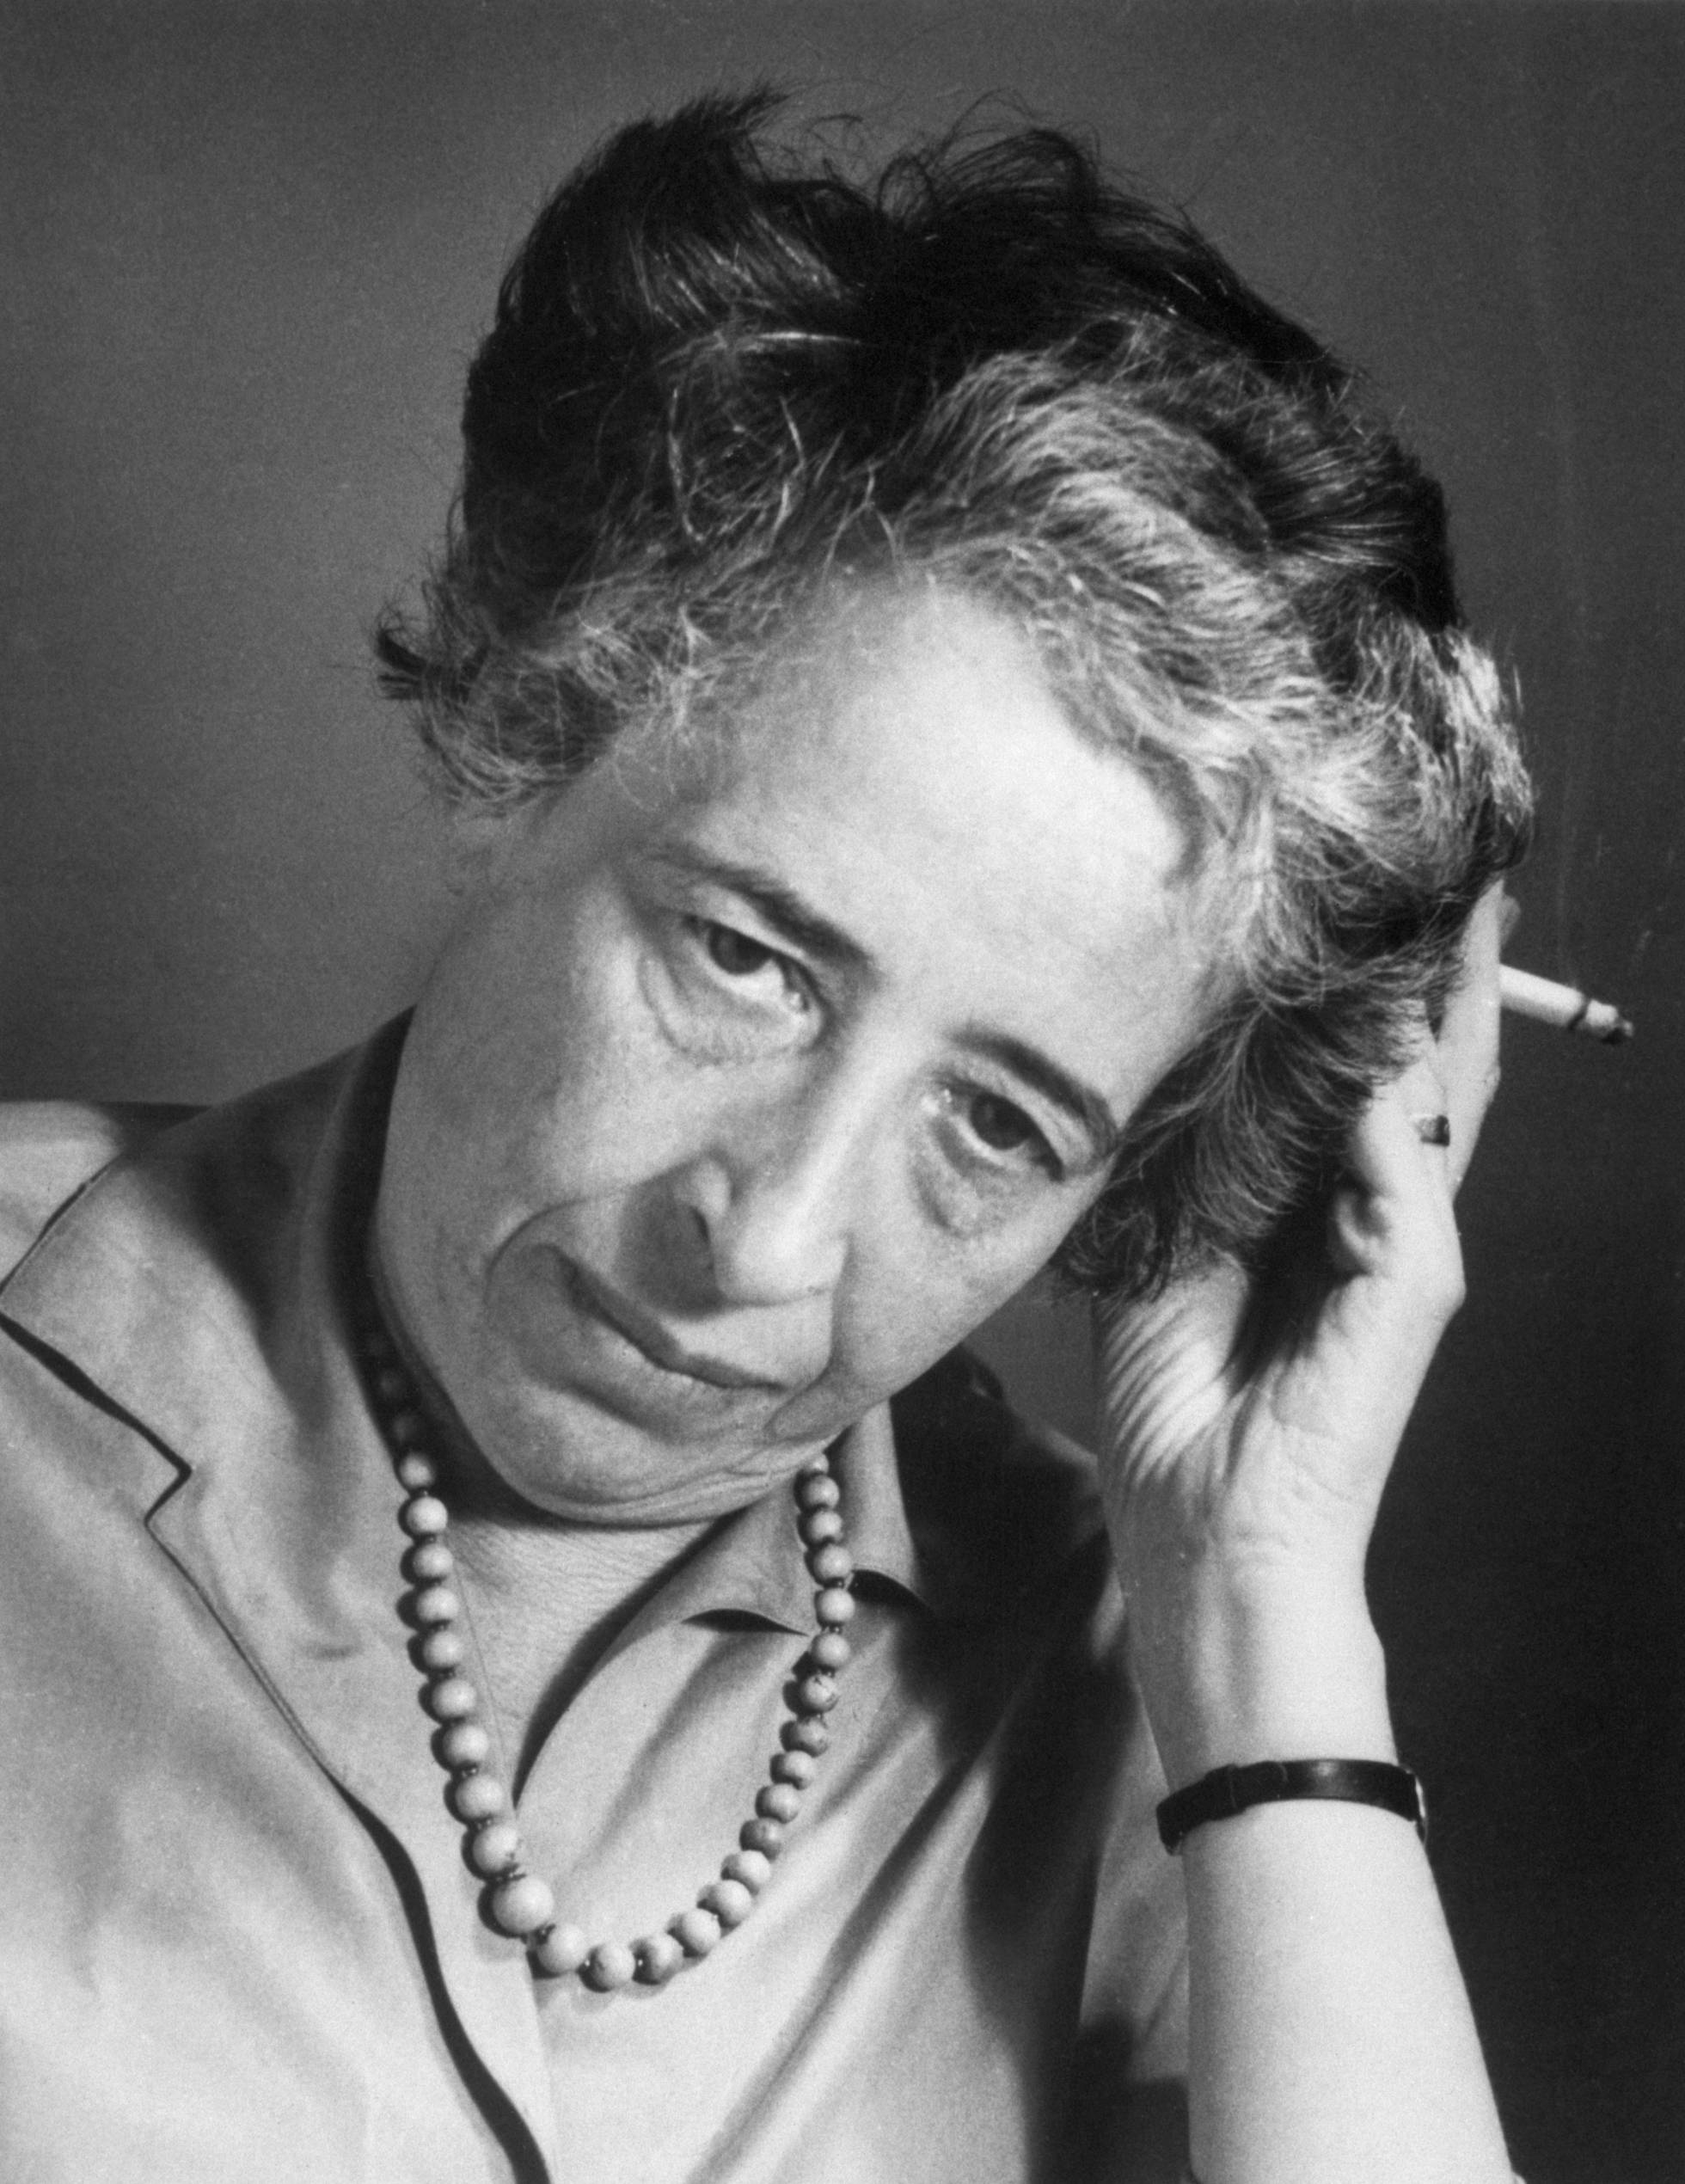
\includegraphics[width = 0.9\textwidth]{img/arendt}\\
% Hannah Arendt,\\\textit{On Violence} (1970)
% \end{minipage}
%
% \end{frame}

% \begin{frame}
% \frametitle{Another key point: violence is usually collective}
% \centering
%
% \begin{itemize}
% \item Why social groups fight each other? Why most confrontations do \textit{not} lead to violence?
% \item Roger Gould: interpersonal violence is a property of relationships, not persons
% \item Role of group solidarity: double-edged sword
% \item Charles Tilly:
% \end{itemize}
%
% Tilly
%
% Gould
%
% \end{frame}

\begin{frame}
\frametitle{Course logistics}
\centering

\begin{itemize}
\item Lecture (Thu)
  \begin{itemize}
    \item Main concepts and debates
    \item Reading not mandatory
  \end{itemize}
\item Seminar (Fri)
  \begin{itemize}
    \item We'll discuss a lighter reading (\textit{mandatory})
    \item Group presentation
  \end{itemize}
\item All readings in \textit{Aula Global}
\item All slides in \href{https://franvillamil.github.io/wp_polvio/}{franvillamil.github.io/wp\_polvio/}
\end{itemize}

\end{frame}

% ----------------------------------------------------
\begin{frame}
\frametitle{Evaluation}
\centering

\begin{itemize}
\item Attendance \& participation in seminars (10\%)
\item Presentation (15\%)
\item Reading memos (15\%)
\item Final exam (60\%): 2 options
\end{itemize}

\end{frame}
% ----------------------------------------------------

% ----------------------------------------------------
\begin{frame}
\frametitle{Group presentation}
\centering

\begin{itemize}
  \item Groups of 3-4 people
  \item Choose a week of the course (first come, first served) and choose a related topic (ask me)
  \item 15-minute presentation
  \item Last week: extra presentations with penalty
\end{itemize}

\end{frame}
% ----------------------------------------------------

% ----------------------------------------------------
\begin{frame}
\frametitle{Reading memos}
\centering

\begin{itemize}
  \item Half-page comment on the seminar readings (no summary)
  \item Up to three, choose any week except the ones you present on
  \item Send it by email (or hind it in) \textbf{before class} on Fridays
\end{itemize}

\end{frame}
% ----------------------------------------------------

\begin{frame}
\frametitle{Two options for the final exam}
\centering

\begin{itemize}
\item[1.] Take-home exam, 24h to complete it
\item[] 2 open questions, one short and one long (500 and 1000 words max)
\item[]
\item[2.] Read a book and write a review
\item[] Max 2,500 words, due on exam day
\item[] \textit{Not} a summary, but a commentary linking it to what we discussed in class (including readings)
\item[] A few pre-approved options
\end{itemize}

\end{frame}


\begin{frame}
\frametitle{Book review ideas}
\centering

\begin{minipage}{0.45\textwidth}\centering
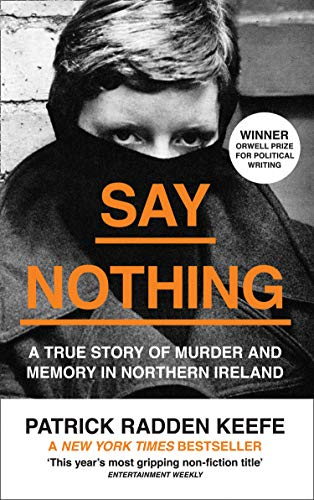
\includegraphics[width = 0.95\textwidth]{img/say_nothing}
\end{minipage}\hfill
\begin{minipage}{0.45\textwidth}\centering
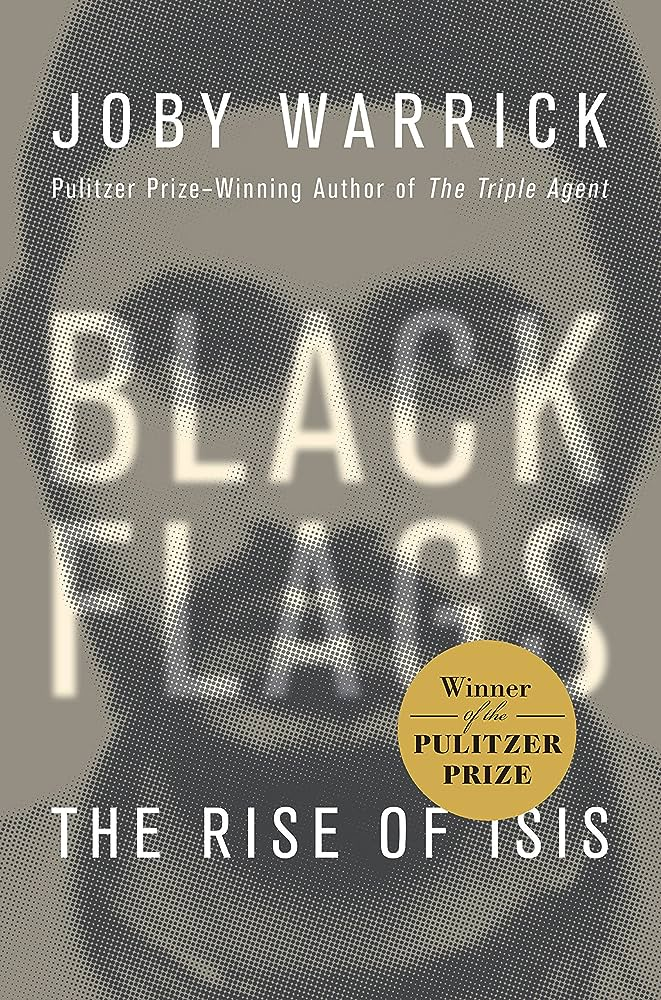
\includegraphics[width = 0.95\textwidth]{img/blackflags}
\end{minipage}

\end{frame}


\begin{frame}
\frametitle{Book review ideas}
\centering

\begin{minipage}{0.45\textwidth}\centering
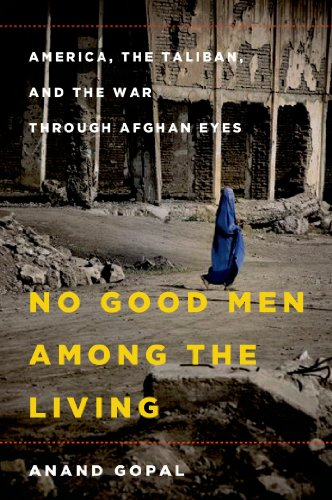
\includegraphics[width = 0.95\textwidth]{img/no_good_men}
\end{minipage}\hfill
\begin{minipage}{0.45\textwidth}\centering
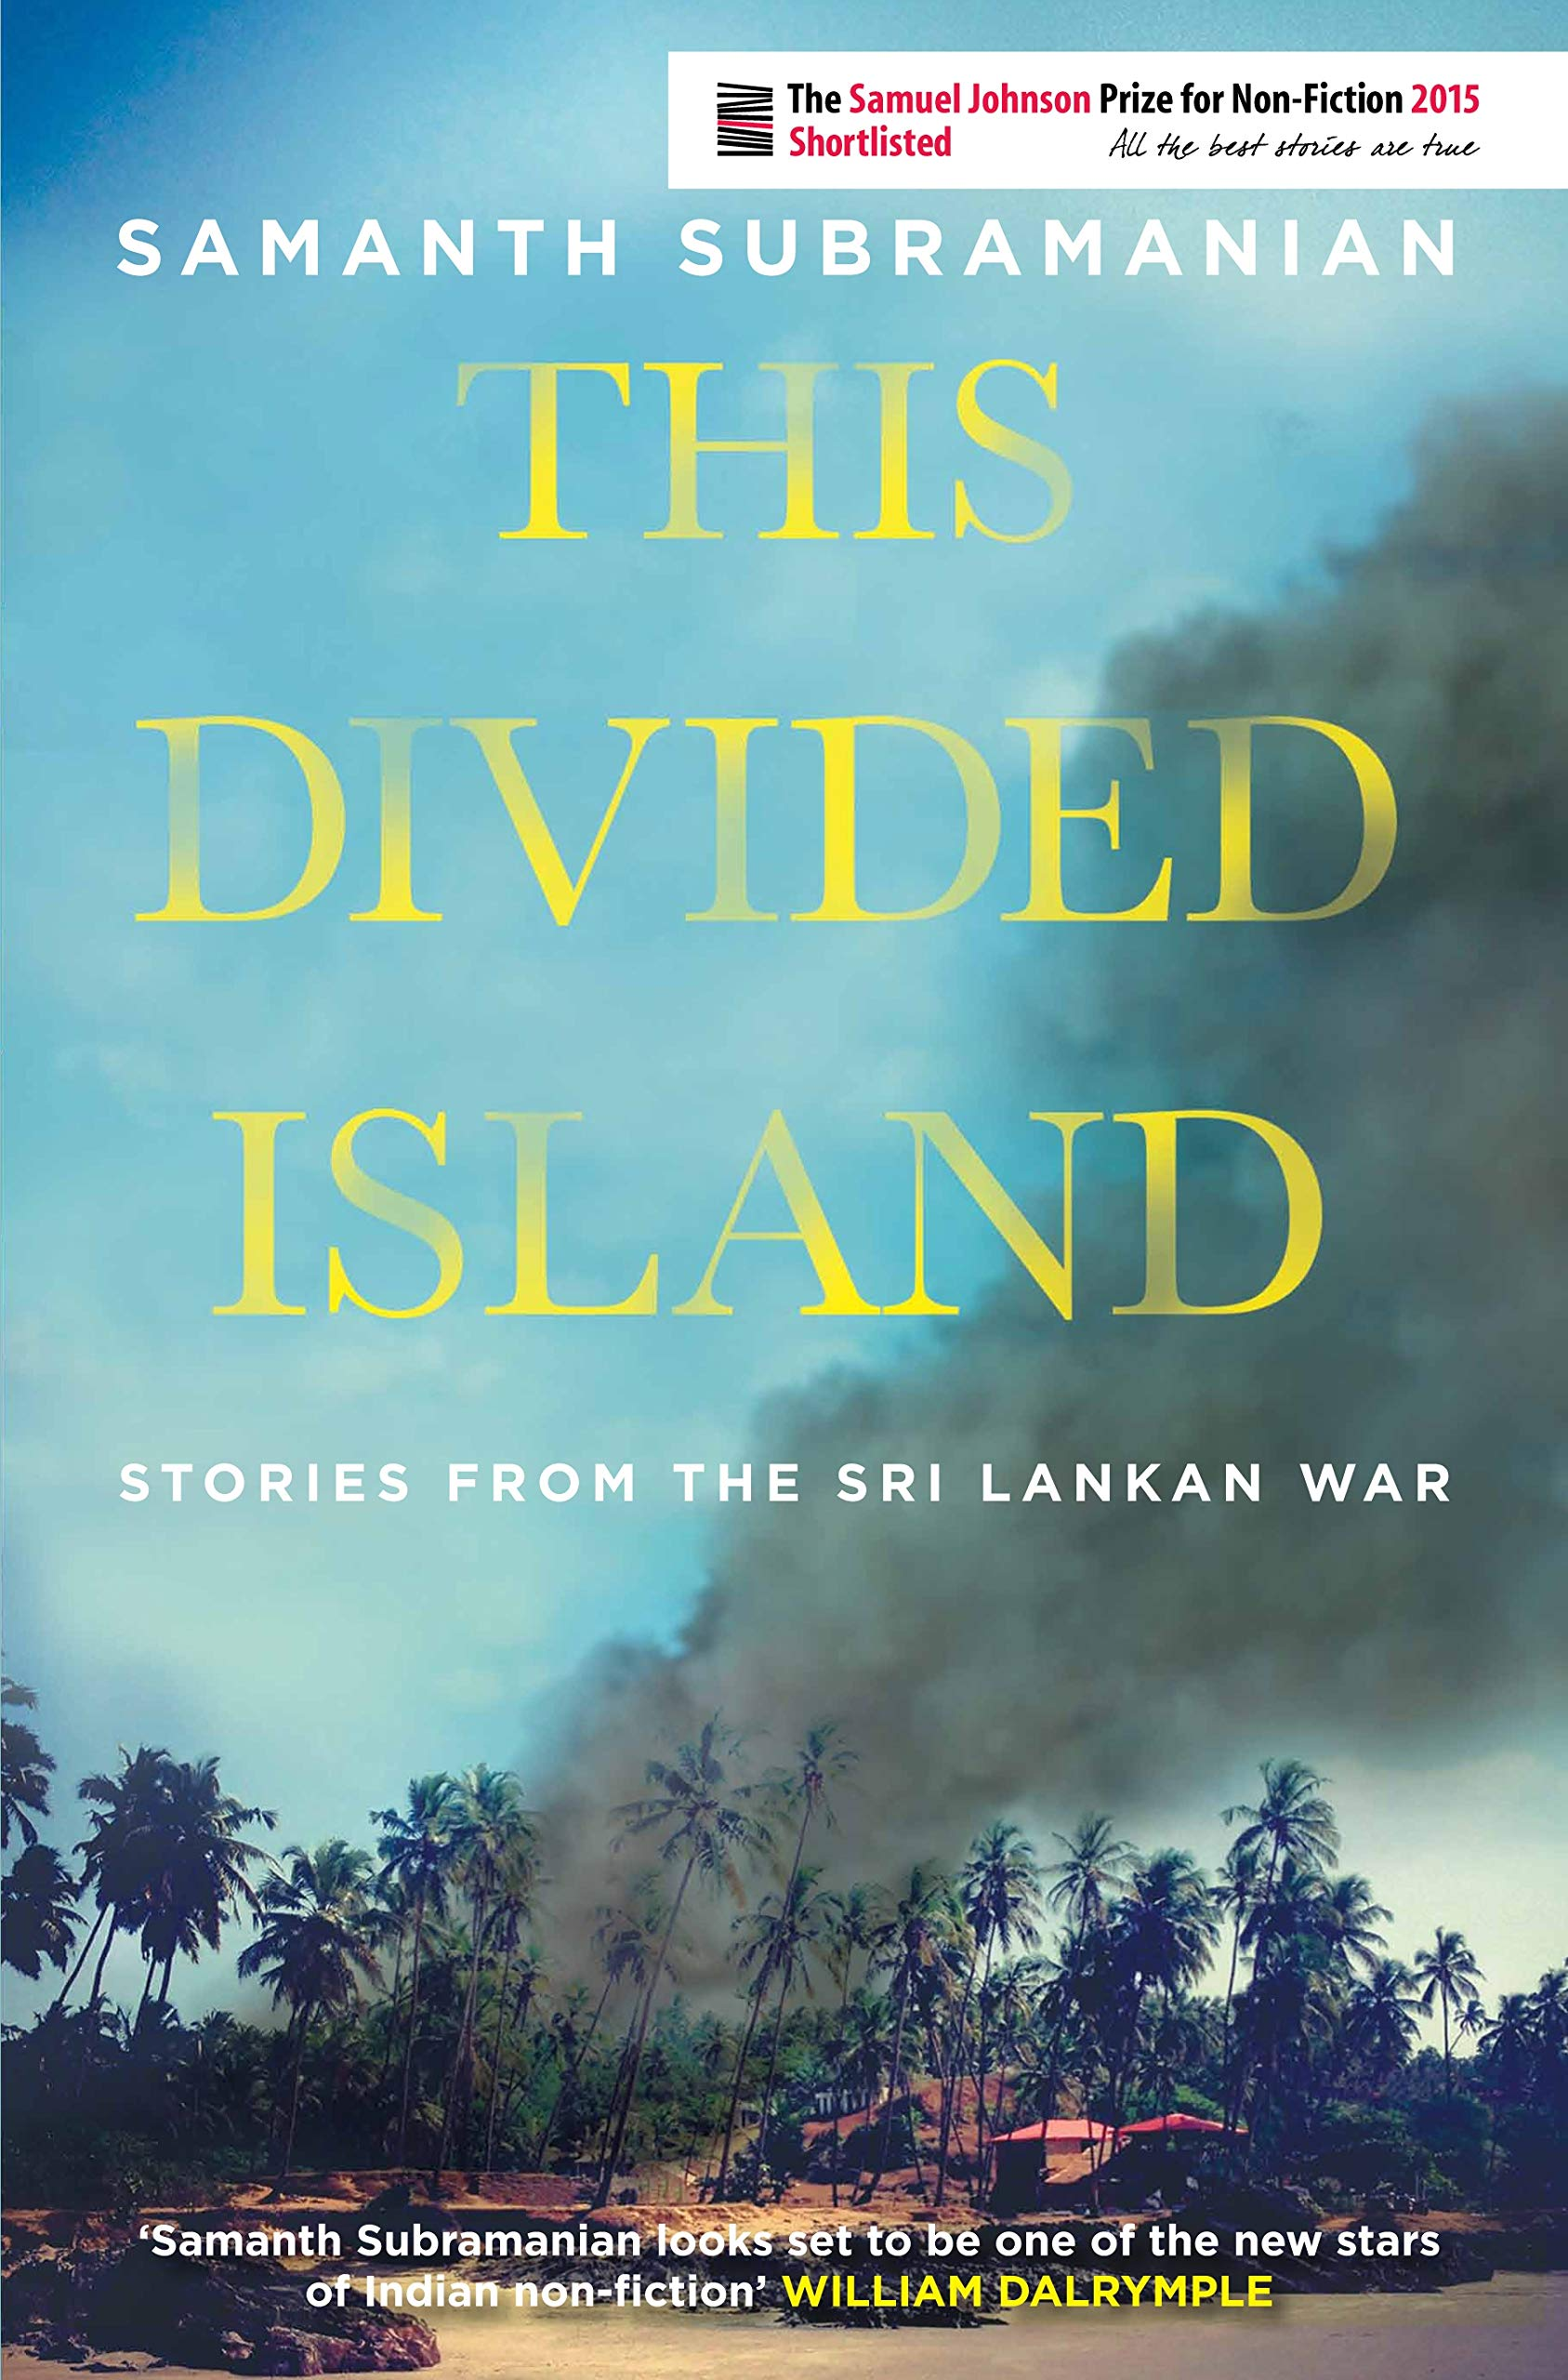
\includegraphics[width = 0.95\textwidth]{img/this_divided_island}
\end{minipage}

\end{frame}


\begin{frame}
\frametitle{Book review ideas}
\centering

\begin{minipage}{0.45\textwidth}\centering
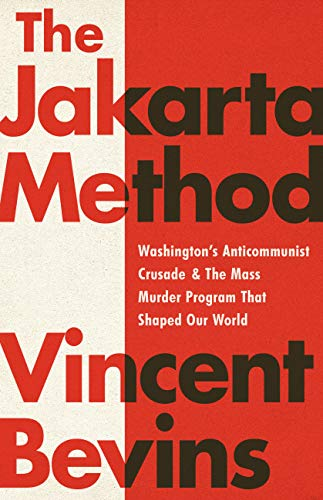
\includegraphics[width = 0.95\textwidth]{img/jakarta_bevins}
\end{minipage}\hfill
\begin{minipage}{0.45\textwidth}\centering
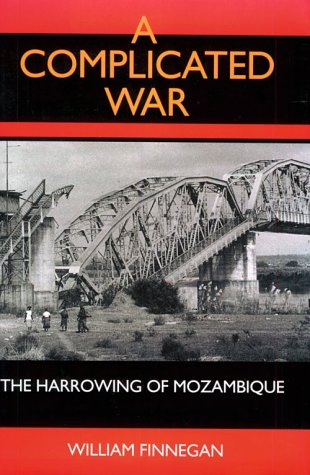
\includegraphics[width = 0.95\textwidth]{img/finnegan_mozambique}
\end{minipage}

\end{frame}

% ----------------------------------------------------
\begin{frame}
\frametitle{}
\centering

\begin{itemize}
  \item \textbf{No class tomorrow (Sept 8)}
  \begin{itemize}
    \item use the time to form groups and choose week
  \end{itemize}
  \item Questions?
\end{itemize}

\end{frame}
% ----------------------------------------------------

\end{document}
